\section{Installazione}
Per utilizzare l'applicazione web è necessario:
\begin{itemize}
\item Clonare la repository (\textbf{Obbligatorio});
\item Importare il database (\textit{Opzionale});
\item Avviare il server (\textit{Opzionale});
\item Avviare la web app (\textbf{Obbligatorio}).
\end{itemize}
\subsection{Clonare la repository}
\begin{enumerate}[label=\textbf{\arabic*})]
	\item Scaricare il codice come file .zip direttamente dal repository CodeBusters-HDViz:
		\begin{center}
			\textcolor{blue}{\url{https://github.com/CodeBusterswe/CodeBusters-HDviz}}
		\end{center}	
	Oppure, con \glo{Git} installato in locale, è possibile clonare il repository con il comando:
		\begin{center}
			\textcolor{coloreRosso}{\textbf{git clone https://github.com/CodeBusterswe/CodeBusters-HDviz}}
		\end{center}
      
	\item Localizzare da terminale la cartella in cui si è stato estratto/clonato il prodotto:  
		\begin{center}
			\textcolor{coloreRosso}{\textbf{cd percorso\textbackslash CodeBusters-HDViz}}
 		\end{center}
\end{enumerate}
\subsection{Importare il database}
\begin{enumerate}[label=\textbf{\arabic*})]
\item Installare PostegreSQL e pgAdmin dal sito:
	\begin{center}
			\textcolor{blue}{\url{https://www.postgresql.org/download/}}
	\end{center}	
\item Creare un nuovo database;
\item Fare il restore del database utilizzando il file \textbf{dumbDB.js} presente nella cartella \texttt{server} del prodotto.
\end{enumerate}
\subsection{Avviare il server}
\begin{enumerate}[label=\textbf{\arabic*})]
\item Entrare nella cartella \texttt{server} con il comando:
	\begin{center}
			\textcolor{coloreRosso}{\textbf{cd server}}
 	\end{center}
\item Nel caso di primo avvio, digitare:
	\begin{center}
			\textcolor{coloreRosso}{\textbf{npm install}}
 	\end{center}
\item Controllare che i valori impostati nel file \textbf{default.js} nella sottocartella \texttt{config} corrispondano a quelli impostati in PostegreSQL:
\begin{itemize}
\item 'USER\underline{}NAME' : nome utente dell'account;
\item 'PASSWORD' : password dell'account;
\item 'HOST' : porta di postegreSQL;
\item 'DB\_NAME' : nome del database precedentemente creato;
\end{itemize}
\item Avviare il server con il comando:
	\begin{center}
			\textcolor{coloreRosso}{\textbf{npm start}}
 	\end{center}
\end{enumerate}
\subsection{Avviare la web app}
\begin{enumerate}[label=\textbf{\arabic*})]
\item Entrare nella cartella \texttt{client} con il comando:
	\begin{center}
			\textcolor{coloreRosso}{\textbf{cd client}}
 	\end{center}
\item Nel caso di primo avvio digitare il comando:
		\begin{center}
			\textcolor{coloreRosso}{\textbf{npm install}}
 		\end{center}
\item Fare la build dell'app con il comando:
		\begin{center}
			\textcolor{coloreRosso}{\textbf{npm run build}}
 		\end{center}
\item nel caso di primo avvio dell'applicazione sul sistema, digitare:
		\begin{center}
			\textcolor{coloreRosso}{\textbf{npm install -g serve}}
 		\end{center}	     
\item Digitare poi:
		\begin{center}
			\textcolor{coloreRosso}{\textbf{serve -s build -l 4000}}
 		\end{center}		
\end{enumerate}

L'applicazione sarà disponibile aprendo l'indirizzo fornito dal terminale.

\begin{figure}[H]
		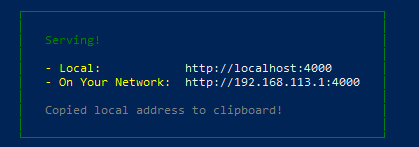
\includegraphics[scale=1]{Images/install.png}
		\centering
		\caption{Avvio dell'applicazione}
\end{figure}
